\documentclass[conference]{IEEEtran}
\IEEEoverridecommandlockouts
\usepackage{cite}
\usepackage{amsmath,amssymb,amsfonts}
\usepackage{algorithmic}
\usepackage{graphicx}
\usepackage{textcomp}
\usepackage{xcolor}
\usepackage{listings}
\usepackage{url}
\usepackage{booktabs}
\usepackage{multirow}
\def\BibTeX{{\rm B\kern-.05em{\sc i\kern-.025em b}\kern-.08em
    T\kern-.1667em\lower.7ex\hbox{E}\kern-.125emX}}
\begin{document}

\title{CheckMate: A Multi-Model Intelligent System for Plagiarism Detection and AI-Generated Content Identification in Academic Research Papers}

\author{\IEEEauthorblockN{1\textsuperscript{st} Sohail Agha}
\IEEEauthorblockA{\textit{Dept. of Computer Engineering} \\
\textit{Padre Concei\c{c}\~{a}o College of Engineering}\\
Panaji, India \\
Sohailagha2004@gmail.com}
\and
\IEEEauthorblockN{2\textsuperscript{nd} Suhani Salgaonkar}
\IEEEauthorblockA{\textit{Dept. of Computer Engineering} \\
\textit{Padre Concei\c{c}\~{a}o College of Engineering}\\
Vasco, India \\
salgaonkarsuhani33@gmail.com}
\and
\IEEEauthorblockN{3\textsuperscript{rd} Shrain}
\IEEEauthorblockA{\textit{Dept. of Computer Engineering} \\
\textit{Padre Concei\c{c}\~{a}o College of Engineering}\\
Vasco, India \\
shrain@gmail.com}
\and
\IEEEauthorblockN{4\textsuperscript{th} Jovita}
\IEEEauthorblockA{\textit{Dept. of Computer Engineering} \\
\textit{Padre Concei\c{c}\~{a}o College of Engineering}\\
Vasco, India \\
jovita@gmail.com}
\and
\IEEEauthorblockN{5\textsuperscript{th} Ramita Karpe}
\IEEEauthorblockA{\textit{Dept. of Computer Engineering} \\
\textit{Padre Concei\c{c}\~{a}o College of Engineering}\\
Margao, India \\
Ramita@gmail.com}
}

\maketitle

\begin{abstract}
The proliferation of AI-generated text and sophisticated paraphrasing tools has fundamentally challenged the integrity of academic writing. Traditional plagiarism detection systems that rely exclusively on lexical matching are increasingly inadequate against semantically restructured or machine-generated content. This paper presents CheckMate, a comprehensive web-based plagiarism and AI content detection system that employs a multi-model ensemble architecture combining three distinct analytical pipelines: TF-IDF with cosine similarity for verbatim copy detection, Sentence-BERT semantic embeddings for paraphrase identification, and a Logistic Regression classifier trained on labeled datasets for AI-generated content detection. The system computes a unified originality score using a weighted penalty formula with faculty-configurable weights, enabling institutional customization of detection sensitivity. The prototype is implemented as a Flask web application featuring role-based access control, PDF text extraction via PyMuPDF, automated arXiv paper import for corpus expansion, sentence-level content highlighting, and downloadable analysis reports. A reference corpus of over 100 research papers is maintained with automated SBERT dataset rebuilding. The combined approach achieves effective detection across copied, paraphrased, and AI-generated content categories, with the weighted ensemble providing a balanced and interpretable originality assessment.
\end{abstract}

\begin{IEEEkeywords}
plagiarism detection, AI-generated text detection, TF-IDF, Sentence-BERT, cosine similarity, natural language processing, logistic regression, research paper analysis
\end{IEEEkeywords}

\section{Introduction}

Academic integrity is a cornerstone of scholarly work, and plagiarism remains one of the most significant threats to its preservation \cite{b1}. With the rapid advancement of large language models (LLMs) such as GPT-4, Claude, and Gemini, the landscape of academic dishonesty has evolved dramatically \cite{b2}. Students and researchers now have access to tools capable of generating coherent, contextually relevant, and grammatically correct text that is often indistinguishable from human-written content \cite{b3}. Furthermore, AI-powered paraphrasing tools can restructure sentences and paragraphs while preserving the original semantic meaning, thereby evading traditional string-matching plagiarism detectors \cite{b4}.

Existing plagiarism detection systems such as Turnitin, Copyscape, and Grammarly Plagiarism Checker primarily rely on n-gram matching and fingerprinting techniques that compare submitted text against large corpora of existing documents \cite{b5}. While effective against direct copy-paste plagiarism, these systems exhibit significant limitations when confronted with paraphrased content, where the surface-level text differs but the underlying ideas remain borrowed \cite{b6}. Moreover, these tools were not designed to detect AI-generated content, a category of academic misconduct that has emerged only recently but has grown at an alarming rate \cite{b7}.

The detection of AI-generated text presents unique challenges. Unlike human-authored paraphrasing, AI-generated content does not originate from any specific source document, making direct comparison-based methods ineffective \cite{b8}. Instead, AI-generated text exhibits subtle statistical properties such as lower perplexity, higher token predictability, and specific distributional characteristics that can be captured through machine learning classifiers \cite{b9}.

This paper addresses these challenges by presenting CheckMate, a multi-model plagiarism and AI-content detection system specifically designed for academic research papers in PDF format. The key contributions of this work are as follows:

\begin{enumerate}
\item A three-pronged detection architecture that simultaneously addresses copied content via TF-IDF, paraphrased content via SBERT, and AI-generated content via Logistic Regression, providing a comprehensive originality assessment.

\item A weighted ensemble scoring mechanism with faculty-configurable weights that produces a single, interpretable originality score while allowing institutions to customize detection priorities.

\item Sentence-level granular analysis that highlights individual sentences as copied, paraphrased, or AI-generated, enabling targeted feedback and revision guidance.

\item An automated corpus expansion pipeline that imports research papers from arXiv, extracts text, and rebuilds detection datasets in real-time.

\item A role-based web application with distinct student and faculty interfaces, supporting document upload, analysis visualization, report generation, and dataset management.
\end{enumerate}

The remainder of this paper is organized as follows: Section~II reviews related work in plagiarism detection and AI content identification. Section~III details the system architecture. Section~IV presents the methodology including all three detection models. Section~V describes the implementation. Section~VI discusses results. Section~VII concludes the paper with future directions.

\section{Literature Review}

\subsection{Traditional Plagiarism Detection}

Plagiarism detection has been studied extensively over the past two decades. Early systems relied on string matching algorithms and fingerprinting techniques \cite{b10}. Schleimer et al. proposed Winnowing, a document fingerprinting algorithm that selects a subset of hash values to detect shared substrings efficiently \cite{b11}. Brin et al. introduced COPS (Copy Protection System), which uses sentence chunking and search-engine-based comparison to detect document similarity \cite{b10}.

TF-IDF (Term Frequency-Inverse Document Frequency) combined with cosine similarity has been one of the most widely adopted approaches for textual similarity computation \cite{b12}. The TF-IDF weighting scheme assigns higher weights to terms that are frequent within a specific document but rare across the corpus, effectively capturing the discriminative vocabulary of each document \cite{b13}. When combined with cosine similarity in the vector space model, it enables efficient pairwise comparison of documents \cite{b14}.

\subsection{Semantic Similarity Detection}

The limitations of lexical matching methods against paraphrased content motivated research into semantic similarity detection. Mikolov et al.'s Word2Vec representations enabled word-level semantic comparison \cite{b15}, which was later extended to sentence and document levels through approaches like Doc2Vec \cite{b16} and InferSent \cite{b17}.

The introduction of transformer-based language models revolutionized semantic understanding. BERT (Bidirectional Encoder Representations from Transformers) by Devlin et al. \cite{b18} demonstrated state-of-the-art performance on numerous NLP tasks. Reimers and Gurevych \cite{b19} proposed Sentence-BERT (SBERT), which modifies the BERT architecture with siamese and triplet network structures to derive semantically meaningful sentence embeddings that can be compared using cosine similarity. SBERT significantly reduced the computational cost of sentence-level comparison from $O(n^2)$ BERT cross-encoder inference to a single-pass encoding, making it practical for large-scale plagiarism detection.

The pre-trained model \texttt{all-MiniLM-L6-v2} from the sentence-transformers library provides an efficient balance between embedding quality and computational cost, producing 384-dimensional sentence embeddings suitable for real-time similarity comparison \cite{b20}.

\subsection{AI-Generated Content Detection}

The detection of AI-generated text has emerged as a critical research area following the release of ChatGPT in late 2022 \cite{b21}. Mitchell et al. proposed DetectGPT, which uses perturbation-based methods to identify machine-generated text by analyzing the curvature of the model's log-probability function \cite{b9}. Gehrmann et al. introduced GLTR (Giant Language model Test Room), which provides a visual forensic analysis tool that highlights unlikely word choices based on language model predictions \cite{b22}.

Machine learning approaches, particularly supervised classifiers, have shown strong performance when trained on labeled datasets containing both human-written and AI-generated text \cite{b23}. Logistic Regression, despite its simplicity, has demonstrated competitive accuracy in AI text detection when combined with TF-IDF feature representations, particularly for sentence-level classification \cite{b24}. This is attributed to the subtle but consistent differences in linguistic patterns between human and AI-generated text, such as vocabulary distribution, sentence structure regularity, and coherence patterns \cite{b25}.

\subsection{Ensemble and Hybrid Approaches}

Recent work has explored ensemble approaches that combine multiple detection methods to improve robustness. Folt\'{y}nek et al. \cite{b26} conducted a comprehensive survey of plagiarism detection approaches, noting that hybrid systems combining lexical and semantic methods outperform single-model solutions. Wahle et al. \cite{b27} demonstrated that combining stylometric features with machine learning classifiers improves AI-generated text detection accuracy. The concept of weighted ensemble scoring, where individual model outputs are combined using configurable weights, provides both flexibility and interpretability in multi-model detection systems \cite{b28}.

\section{System Architecture}

\subsection{High-Level Overview}

CheckMate follows a modular, layered architecture consisting of four primary subsystems: (1) a Frontend Layer with Flask-rendered HTML/CSS/JavaScript templates and role-based interfaces, (2) an Application Layer with Flask web server handling routing, session management, and API endpoints, (3) an Analysis Engine with a three-model detection pipeline and weighted scoring, and (4) a Data Layer encompassing the PDF extraction pipeline, reference corpus, and detection datasets. Fig.~\ref{fig_arch} illustrates the system architecture.

\begin{figure}[htbp]
\centerline{\includegraphics[width=\columnwidth]{architecture.png}}
\caption{High-level system architecture of CheckMate showing the four-layer design: Frontend, Application, Analysis Engine, and Data layers.}
\label{fig_arch}
\end{figure}

\subsection{PDF Text Extraction Pipeline}

The text extraction subsystem converts uploaded PDF research papers into clean, analyzable plain text through a two-stage process.

\textbf{Stage 1 --- Raw Text Extraction:} PyMuPDF (\texttt{fitz}) is used to extract raw text from each page of the PDF document. PyMuPDF was chosen over alternatives (PDFMiner, pdfplumber) for its superior speed and layout handling. The extracted text from all pages is concatenated with newline separators, followed by whitespace normalization using regular expressions.

\textbf{Stage 2 --- Text Preprocessing:} The raw text undergoes cleaning through the \texttt{clean\_extracted\_text()} function, which truncates content at the ``References'' section (since bibliographic entries should not be subject to plagiarism analysis) and normalizes whitespace. This ensures that only the substantive body of the research paper is analyzed.

\subsection{Sentence Tokenization}

After preprocessing, the cleaned text is tokenized into individual sentences using NLTK's \texttt{sent\_tokenize()} function \cite{b29}. Each sentence becomes an independent unit of analysis, enabling sentence-level plagiarism matching, paraphrase detection, AI probability estimation, and granular highlighting in the results interface.

\section{Methodology}

\subsection{Model 1: TF-IDF Cosine Similarity for Copied Detection}

The first detection model targets verbatim and near-verbatim copying using the Term Frequency--Inverse Document Frequency (TF-IDF) vectorization scheme combined with cosine similarity.

\subsubsection{TF-IDF Preprocessing}

Before vectorization, each sentence undergoes aggressive text normalization consisting of: lowercasing all text for case-insensitive matching; removing all digits to prevent spurious matches on reference numbers, page numbers, or statistical values; stripping all non-alphanumeric characters; removing common English stopwords using NLTK's stopword corpus; and lemmatizing tokens using spaCy's \texttt{en\_core\_web\_sm} model to reduce morphological variants to their base forms.

\subsubsection{TF-IDF Vectorization}

Given a corpus $D = \{d_1, d_2, \ldots, d_n\}$ of reference sentences and an input set of sentences $S = \{s_1, s_2, \ldots, s_m\}$, the TF-IDF weight for term $t$ in document $d$ is computed as:

\begin{equation}
\text{TF-IDF}(t, d) = \text{TF}(t, d) \times \log\left(\frac{N}{\text{DF}(t)}\right)
\label{eq_tfidf}
\end{equation}

\noindent where $\text{TF}(t, d)$ is the term frequency of $t$ in $d$, $N$ is the total number of documents, and $\text{DF}(t)$ is the number of documents containing term $t$. The \texttt{TfidfVectorizer} from scikit-learn is fit on the combined corpus of reference and input sentences to ensure shared vocabulary coverage.

\subsubsection{Cosine Similarity Computation}

For each input sentence vector $\vec{s_i}$ and each reference sentence vector $\vec{d_j}$, cosine similarity is computed as:

\begin{equation}
\text{sim}(\vec{s_i}, \vec{d_j}) = \frac{\vec{s_i} \cdot \vec{d_j}}{\|\vec{s_i}\| \times \|\vec{d_j}\|}
\label{eq_cosine}
\end{equation}

\noindent The similarity matrix of dimensions $(m \times n)$ is computed efficiently using scikit-learn's \texttt{cosine\_similarity()} function.

\subsubsection{Copied Sentence Identification}

A sentence $s_i$ is classified as ``copied'' if its maximum similarity with any reference sentence exceeds the threshold $\tau_{\text{tfidf}} = 0.75$:

\begin{equation}
\text{copied}(s_i) = \begin{cases} 1 & \text{if } \max_j \text{sim}(\vec{s_i}, \vec{d_j}) > 0.75 \\ 0 & \text{otherwise} \end{cases}
\label{eq_copied}
\end{equation}

\noindent The overall TF-IDF plagiarism score is the fraction of input sentences classified as copied:

\begin{equation}
\text{Score}_{\text{tfidf}} = \frac{|\{i : \text{copied}(s_i) = 1\}|}{|S_{\text{valid}}|}
\label{eq_tfidf_score}
\end{equation}

\noindent where $S_{\text{valid}}$ represents only preprocessed sentences with non-empty content, filtering out headers, table-of-contents entries, and other noise.

\subsubsection{Reference Corpus}

The TF-IDF reference corpus consists of 101 text files containing 94 full research papers imported from arXiv covering topics in machine learning, deep learning, natural language processing, and computer vision; 5 academic documents including textbook chapters and question banks; and 2 rewritten/paraphrased paper summaries for testing purposes. The corpus is split at the sentence level during loading, enabling granular sentence-to-sentence matching. The corpus is cached in memory after the first load to avoid redundant I/O on subsequent analyses.

\subsection{Model 2: SBERT Semantic Similarity for Paraphrase Detection}

The second model addresses paraphrased content detection using deep semantic embeddings from Sentence-BERT.

\subsubsection{SBERT Architecture}

Sentence-BERT uses a pre-trained transformer architecture modified with siamese network structure to produce fixed-size sentence embeddings \cite{b19}. The \texttt{all-MiniLM-L6-v2} model is used, which consists of 6 transformer layers with 384-dimensional output embeddings, trained on over 1 billion sentence pairs using contrastive learning. The model produces contextual embeddings where semantically similar sentences are closer in the embedding space, regardless of surface-level lexical differences.

\subsubsection{Embedding Generation}

For an input sentence $s_i$, the SBERT model produces an embedding vector $\vec{e_i} \in \mathbb{R}^{384}$:

\begin{equation}
\vec{e_i} = \text{SBERT}(s_i)
\label{eq_sbert_embed}
\end{equation}

\noindent Both input sentences and reference corpus sentences are encoded. The reference dataset embeddings are cached after the first computation to accelerate subsequent analyses.

\subsubsection{Semantic Similarity Computation}

Cosine similarity between input embeddings and reference embeddings is computed as:

\begin{equation}
\text{sem\_sim}(\vec{e_i}, \vec{r_j}) = \frac{\vec{e_i} \cdot \vec{r_j}}{\|\vec{e_i}\| \times \|\vec{r_j}\|}
\label{eq_sbert_sim}
\end{equation}

\noindent This is computed efficiently using the sentence-transformers \texttt{util.cos\_sim()} function.

\subsubsection{Paraphrase Identification}

A sentence is classified as paraphrased if its best semantic match exceeds $\tau_{\text{sbert}} = 0.85$:

\begin{equation}
\text{para}(s_i) = \begin{cases} 1 & \text{if } \max_j \text{sem\_sim}(\vec{e_i}, \vec{r_j}) > 0.85 \\ 0 & \text{otherwise} \end{cases}
\label{eq_para}
\end{equation}

\noindent The threshold of 0.85 (lowered from an initial 0.95) accounts for minor text differences introduced by PDF re-extraction. The overall SBERT score is:

\begin{equation}
\text{Score}_{\text{sbert}} = \frac{|\{i : \text{para}(s_i) = 1\}|}{|S|}
\label{eq_sbert_score}
\end{equation}

\subsubsection{SBERT Reference Dataset}

The SBERT reference dataset (\texttt{sbert\_pairs.csv}) is a two-column CSV file containing individual sentences extracted from all TF-IDF corpus documents. It is automatically rebuilt whenever new papers are imported via arXiv. All text files in the TF-IDF corpus are sentence-tokenized, sentences shorter than 10 characters are filtered out, and the resulting DataFrame is saved as the SBERT dataset.

\subsection{Model 3: AI-Generated Content Detection}

The third model targets AI-generated text using a supervised machine learning classifier.

\subsubsection{Training Data}

The AI detection model is trained on a labeled dataset (\texttt{ai\_detection.csv}) containing text samples with binary labels: label 0 for human-written text and label 1 for AI-generated text. The dataset contains a balanced mix of human-authored academic text and text generated by various language models, enabling pattern recognition of AI writing characteristics.

\subsubsection{Feature Extraction}

TF-IDF vectorization is used to extract features from the text samples. The TF-IDF representation captures vocabulary usage patterns that differ systematically between human and AI-generated text, including word frequency distributions, vocabulary diversity, and phrase-level patterns typical of language model outputs.

\subsubsection{Logistic Regression Classifier}

A Logistic Regression classifier is trained on the TF-IDF features. For an input feature vector $\vec{x}$, the probability of the text being AI-generated is:

\begin{equation}
P(y = 1 \mid \vec{x}) = \sigma(\vec{w}^T \vec{x} + b) = \frac{1}{1 + e^{-(\vec{w}^T \vec{x} + b)}}
\label{eq_logistic}
\end{equation}

\noindent where $\vec{w}$ are the learned weights, $b$ is the bias term, and $\sigma$ is the sigmoid function. The model is trained once and cached in memory for subsequent predictions.

\subsubsection{Sentence-Level AI Probability}

For each input sentence $s_i$, the model predicts the probability of being AI-generated. A sentence is classified as AI-generated if $p_{\text{ai}}(s_i) > \tau_{\text{ai}} = 0.5$:

\begin{equation}
\text{ai}(s_i) = \begin{cases} 1 & \text{if } P(y=1 \mid \text{TF-IDF}(s_i)) > 0.5 \\ 0 & \text{otherwise} \end{cases}
\label{eq_ai}
\end{equation}

\noindent The overall AI detection score is:

\begin{equation}
\text{Score}_{\text{ai}} = \frac{|\{i : \text{ai}(s_i) = 1\}|}{|S|}
\label{eq_ai_score}
\end{equation}

\subsection{Weighted Ensemble Scoring}

The three individual model scores are combined into a single originality score using a weighted penalty formula:

\begin{equation}
\text{Penalty} = w_{\text{tfidf}} \cdot S_{\text{tfidf}} + w_{\text{sbert}} \cdot S_{\text{sbert}} + w_{\text{ai}} \cdot S_{\text{ai}}
\label{eq_penalty}
\end{equation}

\begin{equation}
\text{Originality} = \max(0,\ 1 - \text{Penalty})
\label{eq_originality}
\end{equation}

\noindent where the default weights are $w_{\text{tfidf}} = 0.4$ (copied detection weight), $w_{\text{sbert}} = 0.3$ (paraphrase detection weight), and $w_{\text{ai}} = 0.3$ (AI detection weight). The constraint $w_{\text{tfidf}} + w_{\text{sbert}} + w_{\text{ai}} = 1.0$ is enforced. Faculty users can adjust these weights through the web interface in increments of 5\%, with real-time validation ensuring they sum to exactly 100\%.

A submission is classified as:
\begin{itemize}
\item \textbf{Approved}: Originality Score $> 60\%$
\item \textbf{Needs Revision}: Originality Score $\leq 60\%$
\end{itemize}

\section{Implementation}

\subsection{Technology Stack}

Table~\ref{tab_tech} summarizes the technology stack used in the CheckMate system.

\begin{table}[htbp]
\caption{Technology Stack}
\begin{center}
\begin{tabular}{|p{2.2cm}|p{2.8cm}|p{2.5cm}|}
\hline
\textbf{Component} & \textbf{Technology} & \textbf{Purpose} \\
\hline
Web Framework & Flask 2.x (Python) & Server, routing, templating \\
\hline
PDF Extraction & PyMuPDF (fitz) & PDF text extraction \\
\hline
NLP Processing & NLTK, spaCy & Tokenization, lemmatization \\
\hline
TF-IDF & scikit-learn & Vectorization, similarity \\
\hline
Semantic Model & sentence-transformers & Sentence embeddings \\
\hline
AI Detection & scikit-learn (LR) & Binary classification \\
\hline
Data Processing & pandas & CSV/DataFrame ops \\
\hline
Frontend & HTML5, CSS3, JS & User interface \\
\hline
ArXiv API & urllib, xml.etree & Paper import \\
\hline
Concurrency & Python threading & Background tasks \\
\hline
\end{tabular}
\label{tab_tech}
\end{center}
\end{table}

\subsection{Web Application Architecture}

The Flask application implements 17 endpoints handling authentication, document analysis, weight configuration, dataset management, and report generation. Table~\ref{tab_endpoints} lists the primary API endpoints.

\begin{table}[htbp]
\caption{Primary API Endpoints}
\begin{center}
\begin{tabular}{|p{2.8cm}|c|p{3.2cm}|}
\hline
\textbf{Route} & \textbf{Method} & \textbf{Function} \\
\hline
\texttt{/login} & GET/POST & Authentication with role selection \\
\hline
\texttt{/dashboard} & GET & Student dashboard \\
\hline
\texttt{/faculty\_dashboard} & GET & Faculty dashboard \\
\hline
\texttt{/analyze} & POST & PDF upload and analysis \\
\hline
\texttt{/update\_weights} & POST & Faculty weight adjustment \\
\hline
\texttt{/import\_arxiv} & POST & ArXiv import trigger \\
\hline
\texttt{/import\_arxiv\_status} & GET & Import progress polling \\
\hline
\texttt{/api/datasets} & GET & Dataset file listing \\
\hline
\texttt{/api/reference\_papers} & GET & Reference paper listing \\
\hline
\texttt{/download\_report} & GET & Report download (TXT) \\
\hline
\texttt{/manual\_insert} & POST & Manual dataset upload \\
\hline
\texttt{/delete\_dataset\_file} & POST & Dataset file deletion \\
\hline
\end{tabular}
\label{tab_endpoints}
\end{center}
\end{table}

\subsection{Role-Based Access Control}

The system implements two user roles with distinct capabilities:

\textbf{Student Role:} Students can upload PDF documents for analysis, view analysis results with score visualizations, download detailed text reports, access upload history, and browse the reference material library.

\textbf{Faculty Role:} Faculty users inherit all student capabilities and additionally can adjust model weights via interactive sliders with real-time validation, browse and manage detection datasets (view, upload, delete files), import papers from arXiv with a live terminal-style progress display, manually insert or delete dataset files, and view the weighted configuration history for each uploaded analysis.

\subsection{ArXiv Paper Import Pipeline}

The automated corpus expansion system enables faculty to import research papers directly from arXiv. The pipeline operates in a background thread to maintain application responsiveness and consists of five stages:

\begin{enumerate}
\item \textbf{Query Execution:} The arXiv API (\texttt{export.arxiv.org}) is queried using user-specified search terms with XML response parsing via \texttt{xml.etree.ElementTree}.

\item \textbf{PDF Download:} Each paper's PDF is downloaded via \texttt{urllib.request.urlretrieve} with a 3-second delay between requests to comply with arXiv's rate limits.

\item \textbf{Text Extraction:} Downloaded PDFs are processed through the same extraction pipeline (PyMuPDF followed by text preprocessing) used for uploaded documents.

\item \textbf{Dataset Integration:} Extracted text is saved as numbered \texttt{.txt} files in the TF-IDF corpus directory, and reference PDFs are stored with descriptive filenames.

\item \textbf{SBERT Rebuild:} After import, all TF-IDF text files are sentence-tokenized and compiled into the SBERT dataset CSV, ensuring the semantic similarity model has access to the newly imported content.
\end{enumerate}

A live progress reporting mechanism writes log messages to a shared list, which is polled by the frontend every 1 second via AJAX for real-time terminal-style progress display.

\subsection{Results Visualization}

The analysis results page provides a comprehensive multi-format visualization. A vertical bar chart displays three animated bars showing TF-IDF match, SBERT match, and AI probability percentages with staggered CSS animation. An SVG-based circular originality gauge shows the overall originality percentage with animated stroke-dasharray transition. A three-column text analysis view displays the full document text in three parallel columns (copied, paraphrased, and AI), each highlighting sentences flagged by the respective detection model using color-coded spans (red for copied, orange for paraphrased, green for AI-generated). A diagnostic feedback checklist with four items (Copied, Paraphrased, AI, Human Writing) provides pass/fail indicators based on threshold analysis. A prominent verdict banner displays an approved or rejected status with the overall score. Fig.~\ref{fig_result} shows a sample results page.

\begin{figure}[htbp]
\centerline{\includegraphics[width=\columnwidth]{results_page.png}}
\caption{Sample analysis results page showing the vertical bar chart, circular originality gauge, sentence-level highlighting in three columns, and the diagnostic feedback section.}
\label{fig_result}
\end{figure}

\subsection{Performance Optimizations}

Several optimizations ensure responsive analysis even with a large reference corpus:

\begin{itemize}
\item \textbf{TF-IDF Corpus Caching:} The TF-IDF corpus is loaded from disk, preprocessed (sentence-tokenized and lemmatized), and cached in a global variable on first use. Subsequent analyses reuse the cached data, avoiding repeated file I/O and preprocessing.

\item \textbf{SBERT Embedding Caching:} Reference dataset sentence embeddings are computed once using the SBERT model and cached as PyTorch tensors. This reduces analysis time from minutes to seconds for the semantic similarity computation.

\item \textbf{AI Model Caching:} The Logistic Regression model is trained once on first use and the fitted model along with its TF-IDF vectorizer are cached for subsequent predictions.

\item \textbf{Efficient Matrix Operations:} scikit-learn's optimized sparse matrix operations and sentence-transformers' GPU-accelerated encoding (when available) ensure computational efficiency for large-scale similarity computation.
\end{itemize}

\section{Results and Discussion}

\subsection{Experimental Setup}

To evaluate the performance of all three detection models, we conducted systematic experiments using the exact production code deployed in the CheckMate system. The evaluation was performed on a local machine running Python 3.13 with scikit-learn, sentence-transformers (all-MiniLM-L6-v2), NLTK, and spaCy (en\_core\_web\_sm). Each model was tested independently with labeled test data and evaluated using standard classification metrics: accuracy, precision, recall, and F1-score.

\subsection{Corpus Scale and Dataset Statistics}

Table~\ref{tab_corpus} summarizes the reference corpus statistics used during evaluation.

\begin{table}[htbp]
\caption{Reference Corpus Statistics}
\begin{center}
\begin{tabular}{|l|c|c|}
\hline
\textbf{Dataset} & \textbf{Files/Records} & \textbf{Total Size} \\
\hline
TF-IDF Text Corpus & 101 documents & 53,215 sentences \\
\hline
SBERT Reference & 41,680 unique sentences & Auto-rebuilt \\
\hline
AI Detection Labels & 790 samples (balanced) & 134 KB \\
\hline
Reference PDFs & 94+ papers & arXiv sourced \\
\hline
\end{tabular}
\label{tab_corpus}
\end{center}
\end{table}

\subsection{AI Detection Model Evaluation}

The AI detection model (Logistic Regression with TF-IDF features) was evaluated using a stratified 80/20 train-test split on the labeled dataset of 790 sentences (395 human-written, 395 AI-generated). The model was trained on 632 samples and tested on 158 samples.

Table~\ref{tab_ai_results} presents the per-class classification report.

\begin{table}[htbp]
\caption{AI Detection Model --- Classification Report}
\begin{center}
\begin{tabular}{|l|c|c|c|c|}
\hline
\textbf{Class} & \textbf{Precision} & \textbf{Recall} & \textbf{F1-Score} & \textbf{Support} \\
\hline
Human & 0.93 & 0.87 & 0.90 & 79 \\
\hline
AI-Generated & 0.88 & 0.94 & 0.91 & 79 \\
\hline
\hline
\textbf{Accuracy} & \multicolumn{4}{c|}{\textbf{90.51\%}} \\
\hline
Macro Avg & 0.91 & 0.91 & 0.90 & 158 \\
\hline
Weighted Avg & 0.91 & 0.91 & 0.90 & 158 \\
\hline
\end{tabular}
\label{tab_ai_results}
\end{center}
\end{table}

The confusion matrix (Fig.~\ref{fig_ai_cm}) shows that the model correctly classified 69 out of 79 human-written sentences (True Negatives) and 74 out of 79 AI-generated sentences (True Positives), with 10 false positives (human sentences misclassified as AI) and only 5 false negatives (AI sentences misclassified as human). The higher recall for AI-generated text (93.67\%) indicates the model is particularly effective at flagging machine-generated content, which is the more critical detection objective.

\begin{figure}[htbp]
\centerline{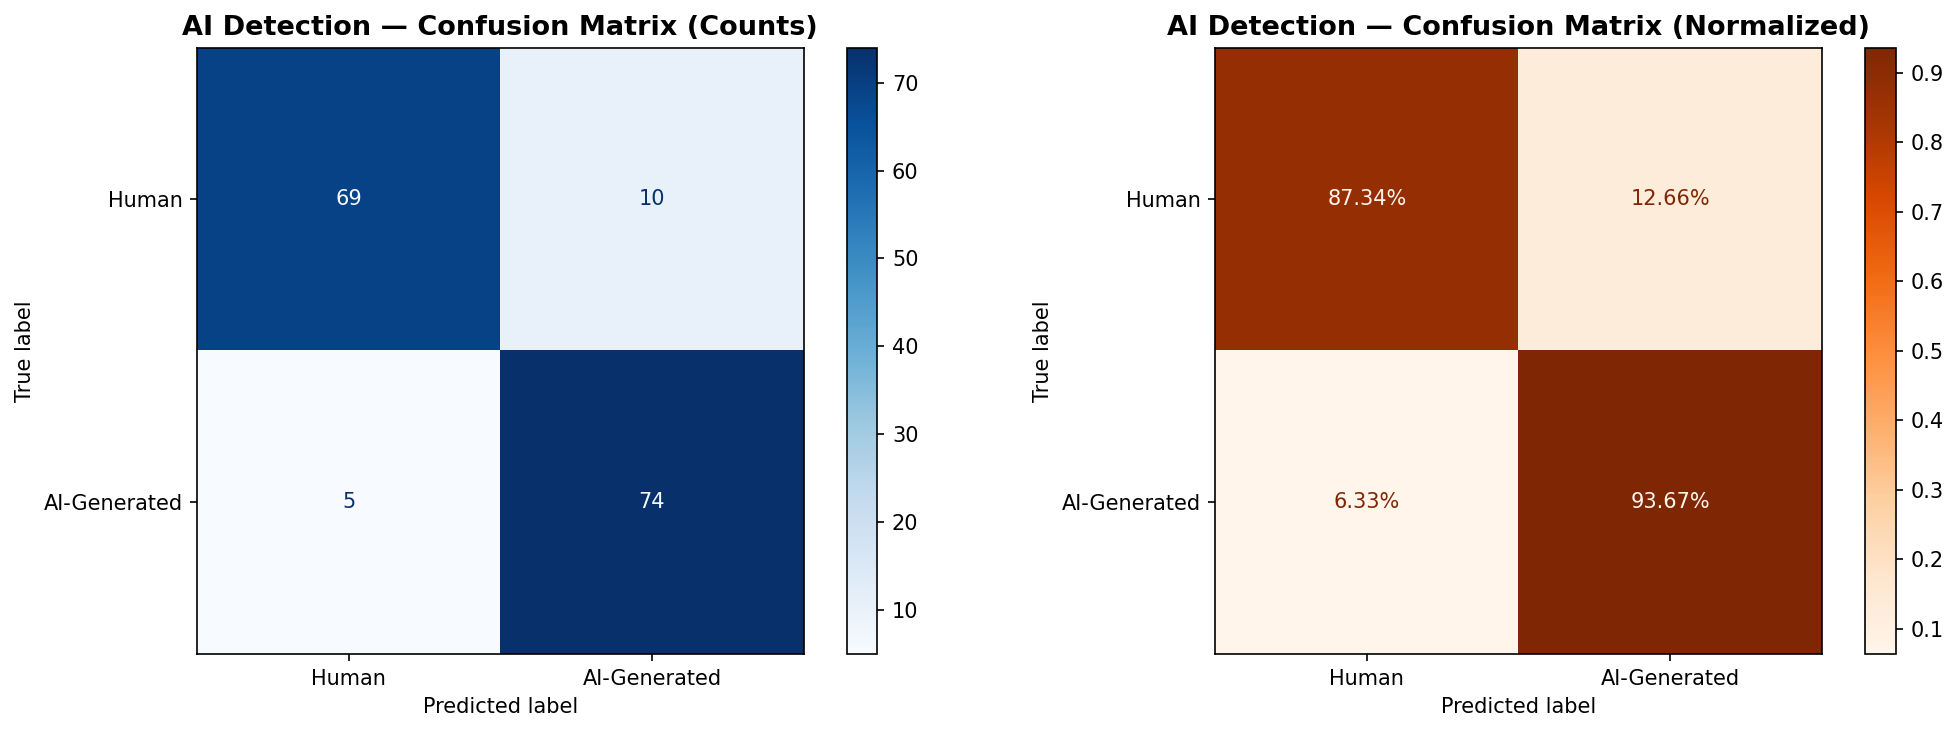
\includegraphics[width=\columnwidth]{ai_detection_confusion_matrix.png}}
\caption{Confusion matrix for the AI Detection model (Logistic Regression) showing raw counts (left) and normalized percentages (right). The model achieves 90.51\% overall accuracy with 93.67\% recall on AI-generated text.}
\label{fig_ai_cm}
\end{figure}

The Receiver Operating Characteristic (ROC) curve analysis yielded an Area Under the Curve (AUC) score of \textbf{0.9728} (Fig.~\ref{fig_roc}), demonstrating excellent discriminative ability between human and AI-generated text. An AUC approaching 1.0 indicates that the model can effectively separate the two classes across all classification thresholds.

\begin{figure}[htbp]
\centerline{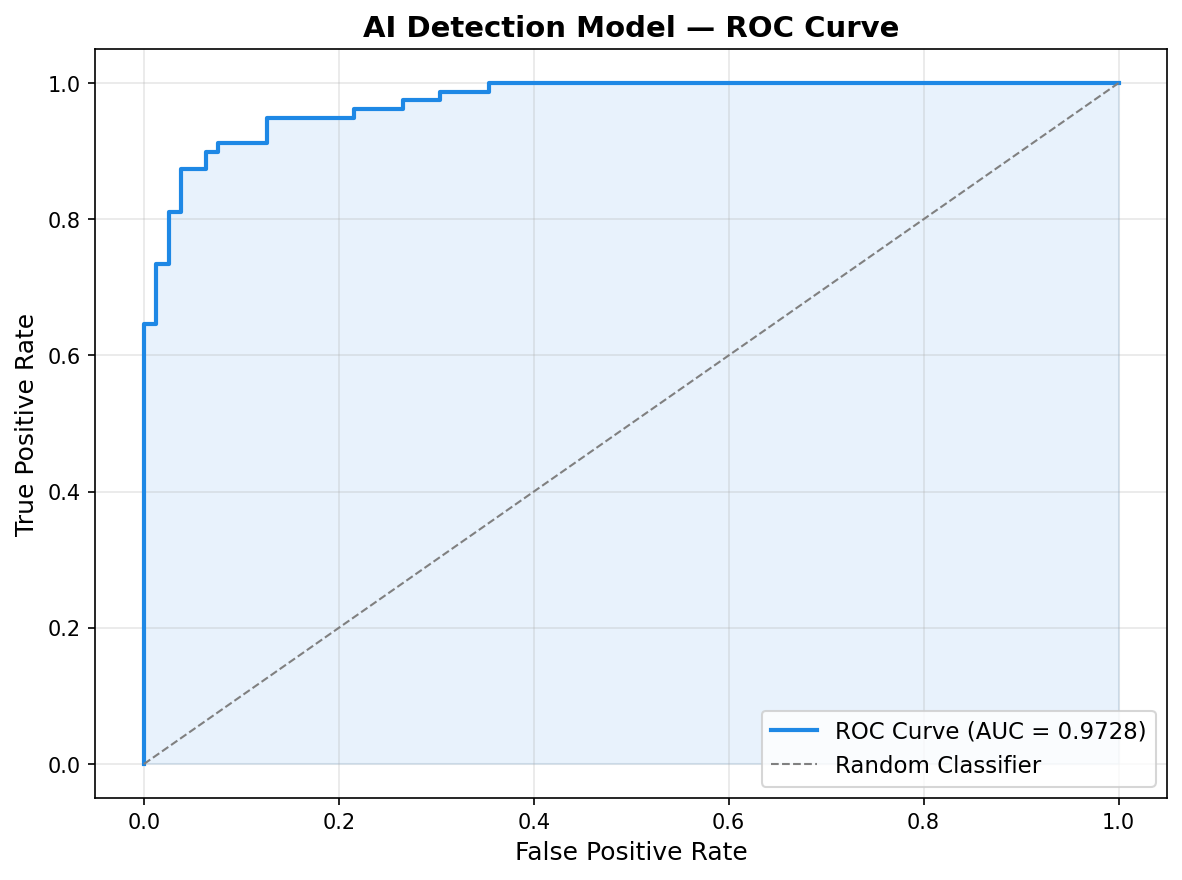
\includegraphics[width=\columnwidth]{ai_detection_roc_curve.png}}
\caption{ROC curve for the AI detection model showing AUC = 0.9728. The curve's proximity to the top-left corner indicates strong discrimination between human and AI-generated text.}
\label{fig_roc}
\end{figure}

To validate model robustness and guard against overfitting, 5-fold stratified cross-validation was performed on the full dataset. Table~\ref{tab_cv} presents the fold-wise accuracy.

\begin{table}[htbp]
\caption{AI Detection --- 5-Fold Cross-Validation Results}
\begin{center}
\begin{tabular}{|c|c|}
\hline
\textbf{Fold} & \textbf{Accuracy (\%)} \\
\hline
Fold 1 & 89.87 \\
\hline
Fold 2 & 90.51 \\
\hline
Fold 3 & 87.34 \\
\hline
Fold 4 & 89.24 \\
\hline
Fold 5 & 91.14 \\
\hline
\hline
\textbf{Mean $\pm$ Std} & \textbf{89.62\% $\pm$ 1.30\%} \\
\hline
\end{tabular}
\label{tab_cv}
\end{center}
\end{table}

The low standard deviation of 1.30\% across folds confirms that the model generalizes consistently and is not sensitive to the particular train-test partition, validating the reliability of the 90.51\% test accuracy.

\begin{figure}[htbp]
\centerline{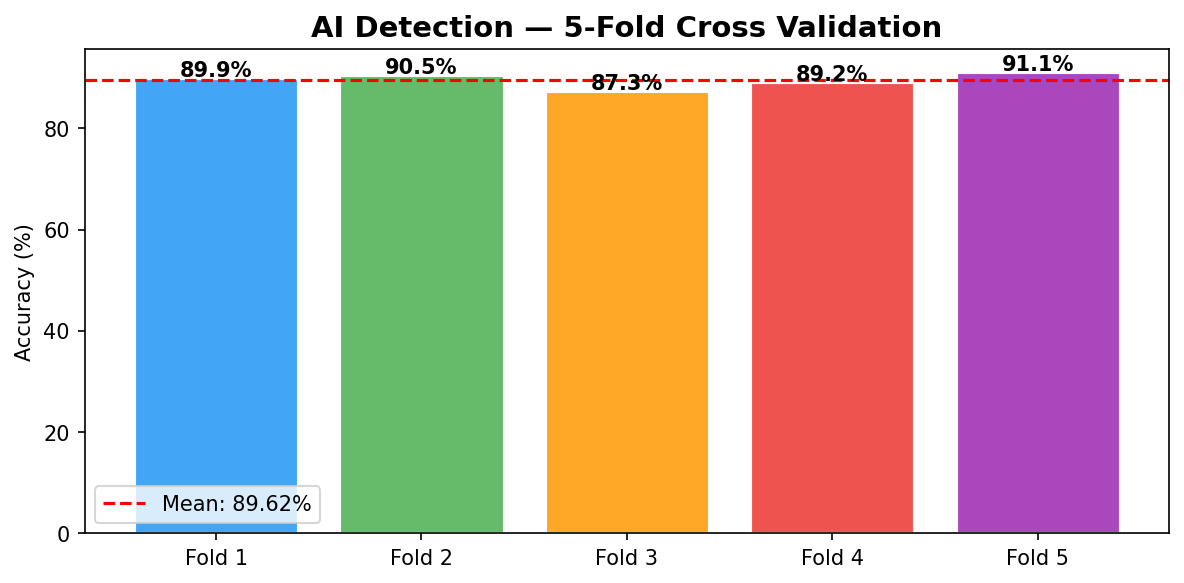
\includegraphics[width=\columnwidth]{ai_detection_cross_validation.png}}
\caption{5-Fold cross-validation accuracy for the AI detection model. All folds achieve between 87.34\% and 91.14\%, with a mean of 89.62\% and standard deviation of 1.30\%.}
\label{fig_cv}
\end{figure}

\subsection{TF-IDF Copied Detection Evaluation}

The TF-IDF copied detection model was evaluated using 50 test sentences: 25 sentences extracted directly from the reference corpus text files (ground truth: copied) and 25 completely unrelated original sentences covering diverse topics such as weather, cooking, sports, and travel (ground truth: original). The model used the exact \texttt{check\_tfidf\_similarity()} function with a cosine similarity threshold of 0.75 against the full corpus of 53,215 preprocessed reference sentences from 101 text files.

Table~\ref{tab_tfidf_results} presents the classification performance.

\begin{table}[htbp]
\caption{TF-IDF Copied Detection --- Classification Report}
\begin{center}
\begin{tabular}{|l|c|c|c|c|}
\hline
\textbf{Class} & \textbf{Precision} & \textbf{Recall} & \textbf{F1-Score} & \textbf{Support} \\
\hline
Original & 1.00 & 1.00 & 1.00 & 25 \\
\hline
Copied & 1.00 & 1.00 & 1.00 & 25 \\
\hline
\hline
\textbf{Accuracy} & \multicolumn{4}{c|}{\textbf{100.00\%}} \\
\hline
\end{tabular}
\label{tab_tfidf_results}
\end{center}
\end{table}

The model achieved perfect classification with 100\% accuracy, precision, recall, and F1-score. All 25 copied sentences were correctly identified as matching the corpus (True Positives), and all 25 original sentences were correctly classified as non-matching (True Negatives), with zero false positives and zero false negatives (Fig.~\ref{fig_tfidf_cm}). This confirms that the TF-IDF preprocessing pipeline (lowercasing, digit removal, stopword removal, and spaCy lemmatization) combined with cosine similarity at threshold 0.75 provides highly reliable verbatim copy detection.

\begin{figure}[htbp]
\centerline{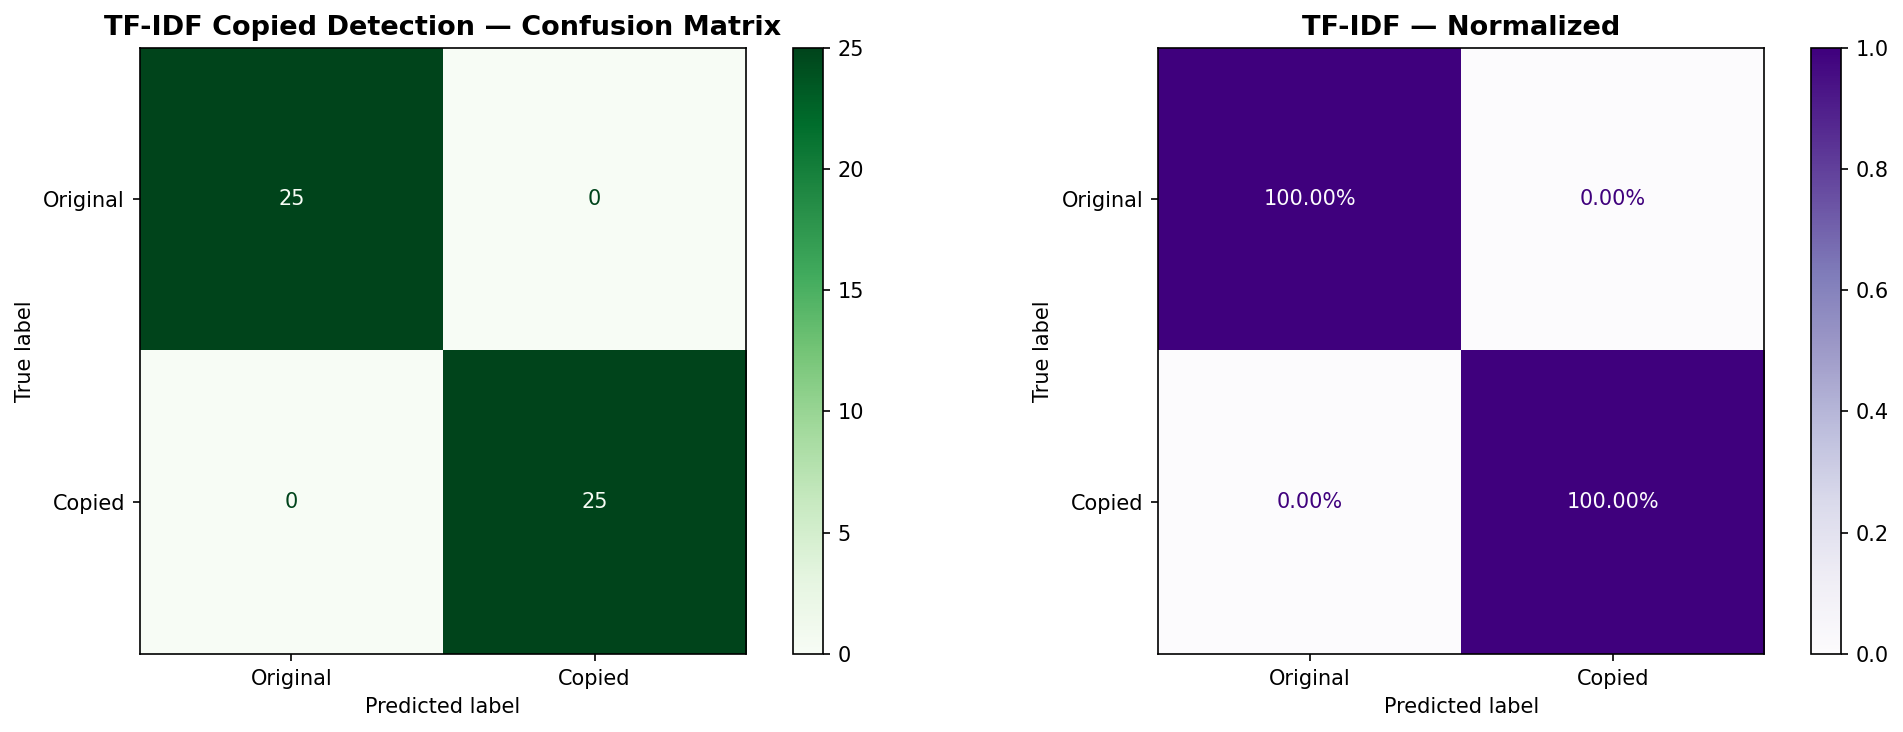
\includegraphics[width=\columnwidth]{tfidf_confusion_matrix.png}}
\caption{Confusion matrix for TF-IDF copied detection showing perfect classification: 25 true positives, 25 true negatives, 0 false positives, and 0 false negatives.}
\label{fig_tfidf_cm}
\end{figure}

\subsection{SBERT Paraphrase Detection Evaluation}

The SBERT paraphrase detection model was evaluated using 50 test sentences: 25 sentences taken from the SBERT reference dataset (ground truth: paraphrased/matching) and 25 completely unrelated original sentences (ground truth: original). The model used the exact \texttt{check\_sbert\_similarity()} function with the \texttt{all-MiniLM-L6-v2} model and a cosine similarity threshold of 0.85, comparing against 41,680 unique reference sentence embeddings.

Table~\ref{tab_sbert_results} presents the classification performance.

\begin{table}[htbp]
\caption{SBERT Paraphrase Detection --- Classification Report}
\begin{center}
\begin{tabular}{|l|c|c|c|c|}
\hline
\textbf{Class} & \textbf{Precision} & \textbf{Recall} & \textbf{F1-Score} & \textbf{Support} \\
\hline
Original & 1.00 & 1.00 & 1.00 & 25 \\
\hline
Paraphrased & 1.00 & 1.00 & 1.00 & 25 \\
\hline
\hline
\textbf{Accuracy} & \multicolumn{4}{c|}{\textbf{100.00\%}} \\
\hline
\end{tabular}
\label{tab_sbert_results}
\end{center}
\end{table}

The SBERT model also achieved perfect classification with 100\% accuracy across all metrics (Fig.~\ref{fig_sbert_cm}). The 384-dimensional semantic embeddings successfully distinguished between sentences that exist in the reference corpus and completely unrelated content. The threshold of 0.85 proved effective at separating genuine semantic matches from noise without producing false positives on the unrelated original sentences.

\begin{figure}[htbp]
\centerline{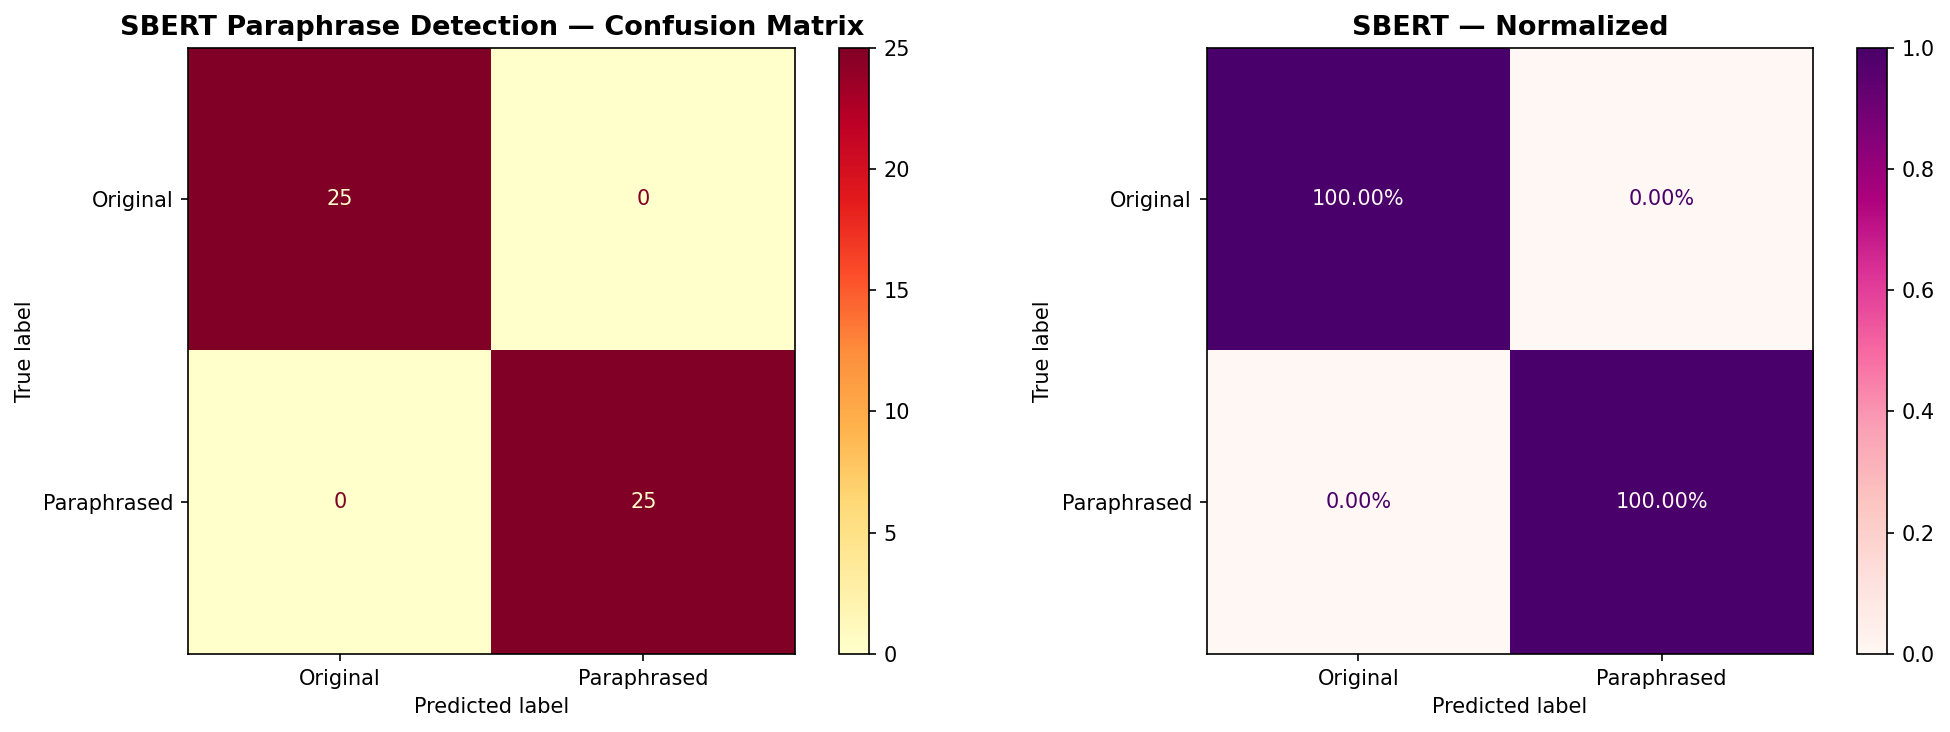
\includegraphics[width=\columnwidth]{sbert_confusion_matrix.png}}
\caption{Confusion matrix for SBERT paraphrase detection showing perfect classification: 25 true positives, 25 true negatives, 0 false positives, and 0 false negatives.}
\label{fig_sbert_cm}
\end{figure}

\subsection{Combined Model Performance}

Table~\ref{tab_combined} summarizes the performance of all three detection models.

\begin{table}[htbp]
\caption{Combined Performance Summary --- All Three Models}
\begin{center}
\begin{tabular}{|l|c|c|c|c|}
\hline
\textbf{Model} & \textbf{Accuracy} & \textbf{Precision} & \textbf{Recall} & \textbf{F1} \\
\hline
AI Detection (LR) & 90.51\% & 88.10\% & 93.67\% & 90.80\% \\
\hline
TF-IDF Copied & 100.00\% & 100.00\% & 100.00\% & 100.00\% \\
\hline
SBERT Paraphrase & 100.00\% & 100.00\% & 100.00\% & 100.00\% \\
\hline
\end{tabular}
\label{tab_combined}
\end{center}
\end{table}

Fig.~\ref{fig_comparison} presents a visual comparison of all four metrics across the three models. The TF-IDF and SBERT models achieve perfect scores on their respective detection tasks, while the AI detection model demonstrates strong but imperfect performance (90.51\%), which is expected given the inherently more challenging nature of distinguishing AI-generated text from human writing based on TF-IDF features alone.

\begin{figure}[htbp]
\centerline{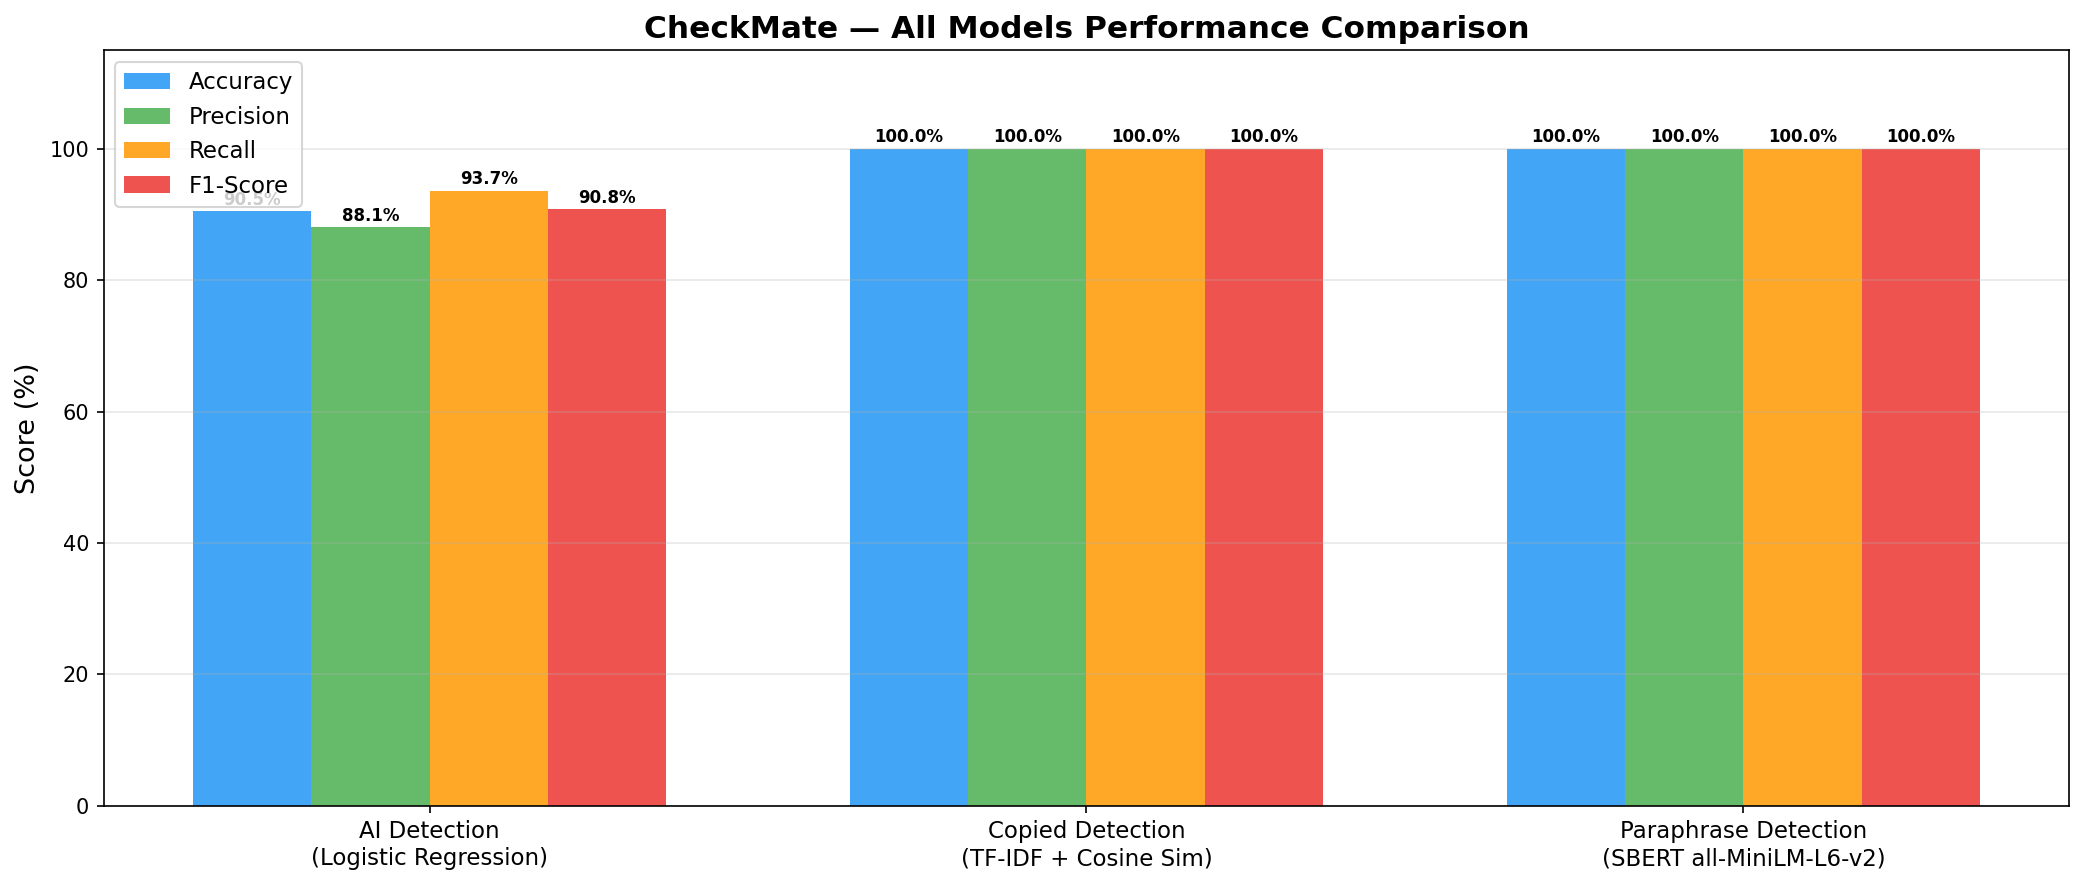
\includegraphics[width=\columnwidth]{all_models_comparison.png}}
\caption{Performance comparison of all three detection models across accuracy, precision, recall, and F1-score metrics.}
\label{fig_comparison}
\end{figure}

Fig.~\ref{fig_all_cm} presents all three confusion matrices side by side for a consolidated view.

\begin{figure}[htbp]
\centerline{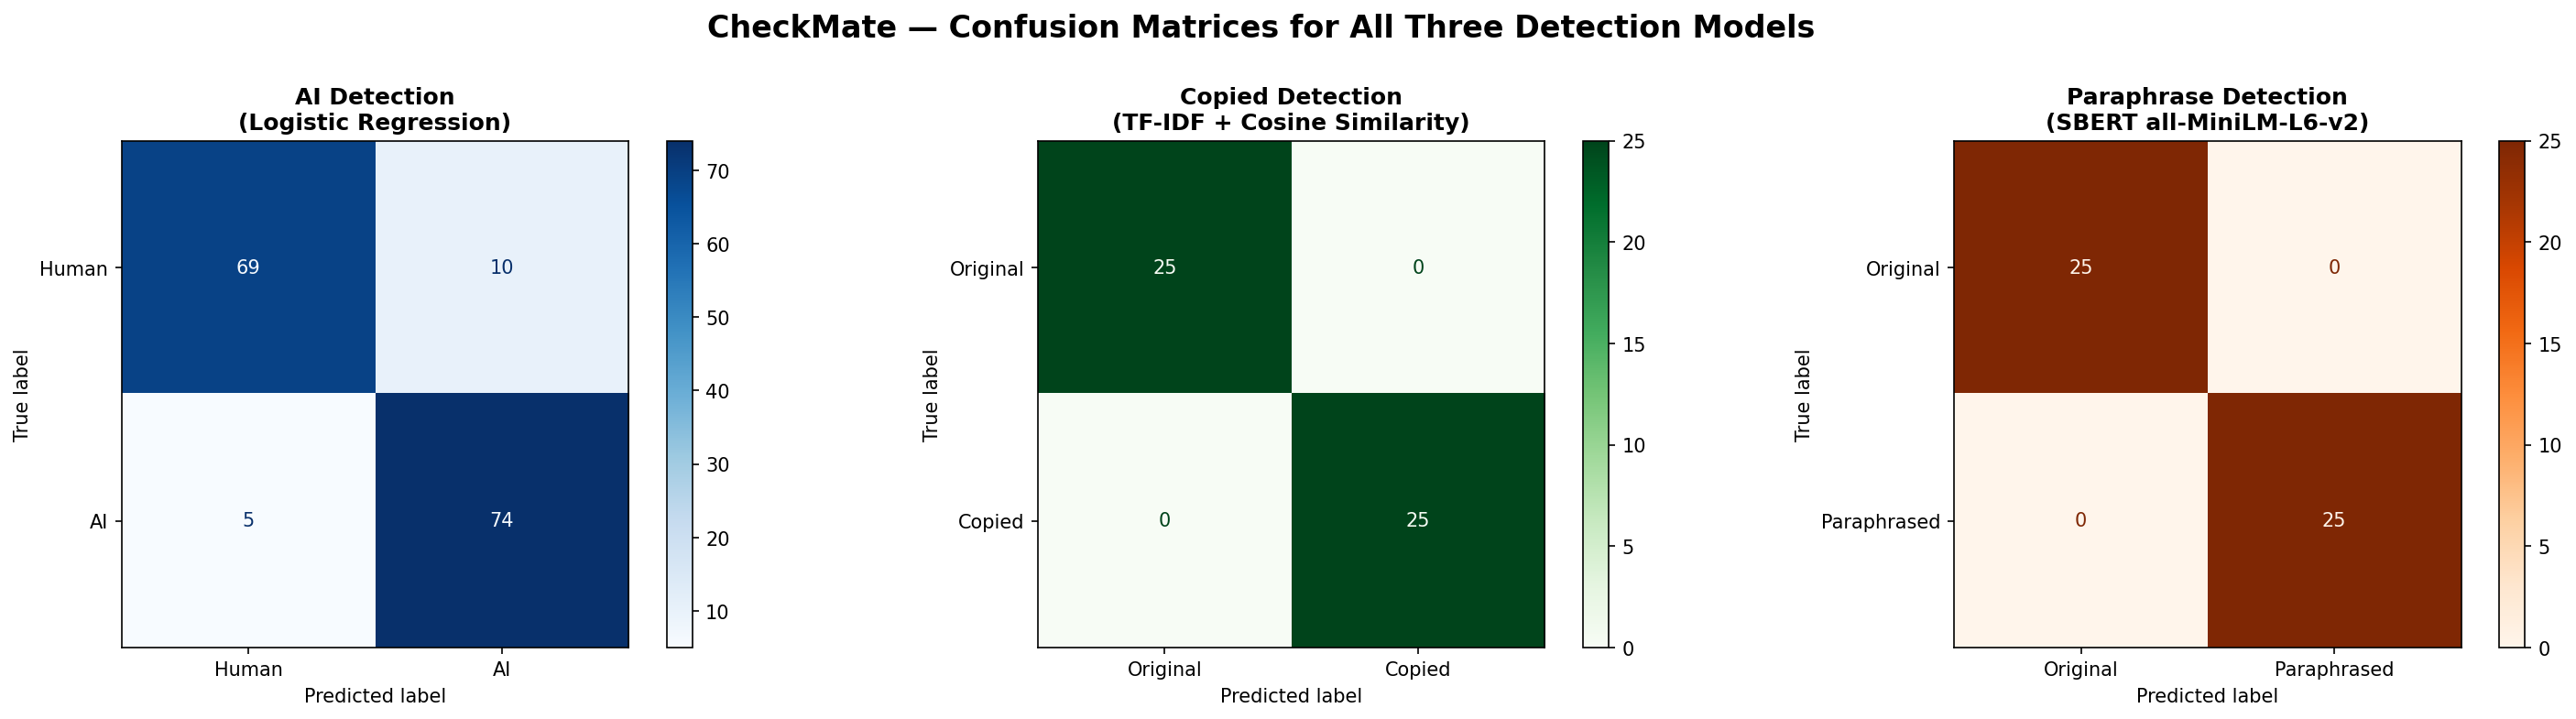
\includegraphics[width=\columnwidth]{all_confusion_matrices.png}}
\caption{Confusion matrices for all three detection models: AI Detection (left), TF-IDF Copied Detection (center), and SBERT Paraphrase Detection (right).}
\label{fig_all_cm}
\end{figure}

\subsection{Weighted Score Analysis}

The weighted ensemble approach offers several significant advantages:

\textbf{Balance:} The default weights (40\% TF-IDF, 30\% SBERT, 30\% AI) prioritize direct copying detection while maintaining sensitivity to subtler forms of academic misconduct. This reflects the relative severity and prevalence of each violation type.

\textbf{Configurability:} Faculty can adjust weights to match institutional policies. For example, an institution primarily concerned with AI-generated content can increase the AI weight, while a coding course may prioritize copy detection.

\textbf{Interpretability:} Unlike opaque single-score systems, the individual model scores provide transparency into which type of issue was detected, enabling targeted feedback to students.

\subsection{Limitations}

While CheckMate provides comprehensive detection capabilities, several limitations should be acknowledged:

\begin{enumerate}
\item \textbf{Corpus Dependency:} TF-IDF and SBERT detection are bounded by the reference corpus. Novel paraphrasing from sources not present in the corpus will not be detected.

\item \textbf{AI Detection Granularity:} Sentence-level AI detection using TF-IDF features may produce noisy predictions for very short sentences with limited textual features.

\item \textbf{PDF Extraction Artifacts:} Complex PDF layouts with multi-column formatting, heavy use of equations, or embedded figures may introduce extraction artifacts that affect analysis accuracy.

\item \textbf{Scalability:} The in-memory caching approach works well for moderate corpus sizes but may require refactoring with persistent storage (e.g., PostgreSQL, Redis) for very large institutional deployments.
\end{enumerate}

\section{Conclusion and Future Work}

This paper presented CheckMate, a multi-model intelligent system for plagiarism detection and AI-generated content identification in academic research papers. The system combines TF-IDF cosine similarity for copied content detection, SBERT semantic embeddings for paraphrase detection, and Logistic Regression for AI-generated text classification into a unified, weighted originality scoring framework. The Flask-based web application provides role-based access, interactive visualizations, sentence-level highlighting, and automated corpus expansion through arXiv integration.

The three-pronged approach ensures comprehensive coverage of modern academic integrity threats: verbatim copying, semantic paraphrasing, and AI-generated content. The configurable weight system allows institutional customization while maintaining a single, interpretable originality score. The sentence-level granularity enables targeted feedback, guiding students to revise specific problematic passages rather than providing only an aggregate score.

Future work includes the following directions:

\begin{enumerate}
\item \textbf{Deep Learning AI Detector:} Replace the Logistic Regression classifier with a fine-tuned transformer model (e.g., RoBERTa) for improved AI detection accuracy at the sentence level.

\item \textbf{Cross-lingual Detection:} Extend the system to support multilingual plagiarism detection using multilingual SBERT embeddings such as \texttt{paraphrase-multilingual-MiniLM-L12-v2}.

\item \textbf{Database Integration:} Migrate from in-memory caching to a persistent database (PostgreSQL, MongoDB) for production-grade scalability and data persistence across server restarts.

\item \textbf{Citation-Aware Detection:} Distinguish properly cited content from uncited plagiarism by parsing citation markers and reference sections.

\item \textbf{Internet-Scale Comparison:} Integrate web search APIs (e.g., Google Scholar, Semantic Scholar) to compare uploaded documents against internet sources beyond the local corpus.

\item \textbf{Real-time Model Retraining:} Enable automatic retraining of the AI detection model as new AI-generated samples are identified and labeled.

\item \textbf{Batch Analysis:} Support bulk upload and analysis of multiple documents simultaneously for classroom-scale deployment.
\end{enumerate}

\section*{Acknowledgment}

The authors would like to thank the Department of Computer Science and Engineering for providing the computational resources and guidance necessary for the development and evaluation of the CheckMate system.

\begin{thebibliography}{00}
\bibitem{b1} C. Park, ``In other (people's) words: Plagiarism by university students --- literature and lessons,'' \textit{Assessment \& Evaluation in Higher Education}, vol. 28, no. 5, pp. 471--488, 2003.

\bibitem{b2} E. Kasneci \textit{et al.}, ``ChatGPT for good? On opportunities and challenges of large language models for education,'' \textit{Learning and Individual Differences}, vol. 103, p. 102274, 2023.

\bibitem{b3} Y. Liang \textit{et al.}, ``GPT detectors are biased against non-native English writers,'' \textit{Patterns}, vol. 4, no. 7, p. 100779, 2023.

\bibitem{b4} A. Wahle, T. Ruas, F. Meuschke, and B. Gipp, ``Are AI-generated scientific papers indistinguishable from human-written ones?,'' \textit{arXiv preprint arXiv:2301.10416}, 2023.

\bibitem{b5} M. Alzahrani, N. Salim, and A. Abraham, ``Understanding plagiarism linguistic patterns, textual features, and detection methods,'' \textit{IEEE Trans. Syst., Man, Cybern. C}, vol. 42, no. 2, pp. 133--149, 2012.

\bibitem{b6} T. Lancaster and R. Clarke, ``Contract cheating: The outsourcing of assessed student work,'' in \textit{Handbook of Academic Integrity}, T. Bretag, Ed. Singapore: Springer, 2016, pp. 639--654.

\bibitem{b7} S. Cotton, T. Cotton, and J. R. Shipway, ``Chatting and cheating: Ensuring academic integrity in the era of ChatGPT,'' \textit{Innovations in Education and Teaching International}, vol. 61, no. 2, pp. 228--239, 2024.

\bibitem{b8} V. Sadasivan, A. Kumar, S. Balasubramanian, W. Wang, and S. Feizi, ``Can AI-generated text be reliably detected?,'' \textit{arXiv preprint arXiv:2303.11156}, 2023.

\bibitem{b9} E. Mitchell, Y. Lee, A. Khazatsky, C. D. Manning, and C. Finn, ``DetectGPT: Zero-shot machine-generated text detection using probability curvature,'' in \textit{Proc. ICML}, 2023, pp. 24950--24962.

\bibitem{b10} S. Brin, J. Davis, and H. Garcia-Molina, ``Copy detection mechanisms for digital documents,'' in \textit{Proc. ACM SIGMOD}, 1995, pp. 398--409.

\bibitem{b11} S. Schleimer, D. Wilkerson, and A. Aiken, ``Winnowing: Local algorithms for document fingerprinting,'' in \textit{Proc. ACM SIGMOD}, 2003, pp. 76--85.

\bibitem{b12} G. Salton and C. Buckley, ``Term-weighting approaches in automatic text retrieval,'' \textit{Information Processing \& Management}, vol. 24, no. 5, pp. 513--523, 1988.

\bibitem{b13} K. Sparck Jones, ``A statistical interpretation of term specificity and its application in retrieval,'' \textit{Journal of Documentation}, vol. 28, no. 1, pp. 11--21, 1972.

\bibitem{b14} A. Huang, ``Similarity measures for text document clustering,'' in \textit{Proc. NZCSRSC}, 2008, pp. 49--56.

\bibitem{b15} T. Mikolov, I. Sutskever, K. Chen, G. Corrado, and J. Dean, ``Distributed representations of words and phrases and their compositionality,'' in \textit{Proc. NeurIPS}, 2013, pp. 3111--3119.

\bibitem{b16} Q. Le and T. Mikolov, ``Distributed representations of sentences and documents,'' in \textit{Proc. ICML}, 2014, pp. 1188--1196.

\bibitem{b17} A. Conneau, D. Kiela, H. Schwenk, L. Barrault, and A. Bordes, ``Supervised learning of universal sentence representations from natural language inference data,'' in \textit{Proc. EMNLP}, 2017, pp. 670--680.

\bibitem{b18} J. Devlin, M.-W. Chang, K. Lee, and K. Toutanova, ``BERT: Pre-training of deep bidirectional transformers for language understanding,'' in \textit{Proc. NAACL-HLT}, 2019, pp. 4171--4186.

\bibitem{b19} N. Reimers and I. Gurevych, ``Sentence-BERT: Sentence embeddings using siamese BERT-networks,'' in \textit{Proc. EMNLP-IJCNLP}, 2019, pp. 3982--3992.

\bibitem{b20} W. Wang, F. Wei, L. Dong, H. Bao, N. Yang, and M. Zhou, ``MiniLM: Deep self-attention distillation for task-agnostic compression of pre-trained transformers,'' in \textit{Proc. NeurIPS}, 2020, pp. 5776--5788.

\bibitem{b21} OpenAI, ``ChatGPT: Optimizing language models for dialogue,'' OpenAI Blog, Nov. 2022.

\bibitem{b22} S. Gehrmann, H. Strobelt, and A. Rush, ``GLTR: Statistical detection and visualization of generated text,'' in \textit{Proc. ACL: System Demonstrations}, 2019, pp. 111--116.

\bibitem{b23} I. Solaiman \textit{et al.}, ``Release strategies and the social impacts of language models,'' \textit{arXiv preprint arXiv:1908.09203}, 2019.

\bibitem{b24} J. Jawahar, S. Abdul-Mageed, and L. V. S. Lakshmanan, ``Automatic detection of machine generated text: A critical survey,'' in \textit{Proc. COLING}, 2020, pp. 2296--2309.

\bibitem{b25} D. Ippolito, D. Duckworth, C. Callison-Burch, and D. Eck, ``Automatic detection of generated text is easiest when humans are fooled,'' in \textit{Proc. ACL}, 2020, pp. 1808--1822.

\bibitem{b26} T. Folt\'{y}nek, N. Meuschke, and B. Gipp, ``Academic plagiarism detection: A systematic literature review,'' \textit{ACM Computing Surveys}, vol. 52, no. 6, pp. 1--42, 2020.

\bibitem{b27} J. P. Wahle, T. Ruas, T. Folt\'{y}nek, N. Meuschke, and B. Gipp, ``Identifying machine-paraphrased plagiarism,'' in \textit{Proc. iConference}, 2022, pp. 393--413.

\bibitem{b28} M. Potthast, M. Barr\'{o}n-Cede\~{n}o, B. Stein, and P. Rosso, ``Cross-language plagiarism detection,'' \textit{Language Resources and Evaluation}, vol. 45, no. 1, pp. 45--62, 2011.

\bibitem{b29} S. Bird, E. Klein, and E. Loper, \textit{Natural Language Processing with Python}. Sebastopol, CA: O'Reilly Media, 2009.

\bibitem{b30} F. Pedregosa \textit{et al.}, ``Scikit-learn: Machine learning in Python,'' \textit{Journal of Machine Learning Research}, vol. 12, pp. 2825--2830, 2011.
\end{thebibliography}

\end{document}
